\documentclass[a4paper]{article}
\usepackage[margin=0.5cm]{geometry}
\pagestyle{empty}
\usepackage[T1]{fontenc}
\usepackage[utf8]{inputenc}
\usepackage{mathptmx}
\usepackage{tikz}
\usetikzlibrary{positioning, arrows.meta, calc, fit, backgrounds}

\definecolor{coreColor}{HTML}{4A90D9}
\definecolor{schedColor}{HTML}{50B848}
\definecolor{attColor}{HTML}{E8533F}
\definecolor{commColor}{HTML}{F5A623}

\tikzset{
    entity header/.style={
        rectangle,
        fill=#1,
        text=white,
        font=\bfseries\footnotesize,
        minimum width=3.6cm,
        minimum height=0.55cm,
        inner sep=2pt,
        anchor=north,
    },
    entity body/.style={
        rectangle,
        fill=#1!5,
        draw=#1,
        line width=0.8pt,
        minimum width=3.6cm,
        inner sep=3pt,
        font=\scriptsize,
        text width=3.2cm,
        anchor=north,
    },
    rel/.style={
        -{Stealth[length=5pt]},
        semithick,
        #1,
    },
    m2m/.style={
        {Stealth[length=5pt]}-{Stealth[length=5pt]},
        semithick,
        #1,
        dashed,
    },
    module label/.style={
        font=\scriptsize\bfseries\itshape,
        text=#1,
    },
}

\newcommand{\entityNode}[5]{%
    \node[entity header=#2] (#1-header) at (#5) {#3};
    \node[entity body=#2, below=0pt of #1-header] (#1-body) {#4};
    \coordinate (#1) at ($(#1-header.north)!0.5!(#1-body.south)$);
    \node[fit=(#1-header)(#1-body), inner sep=0pt] (#1-box) {};
}

\begin{document}
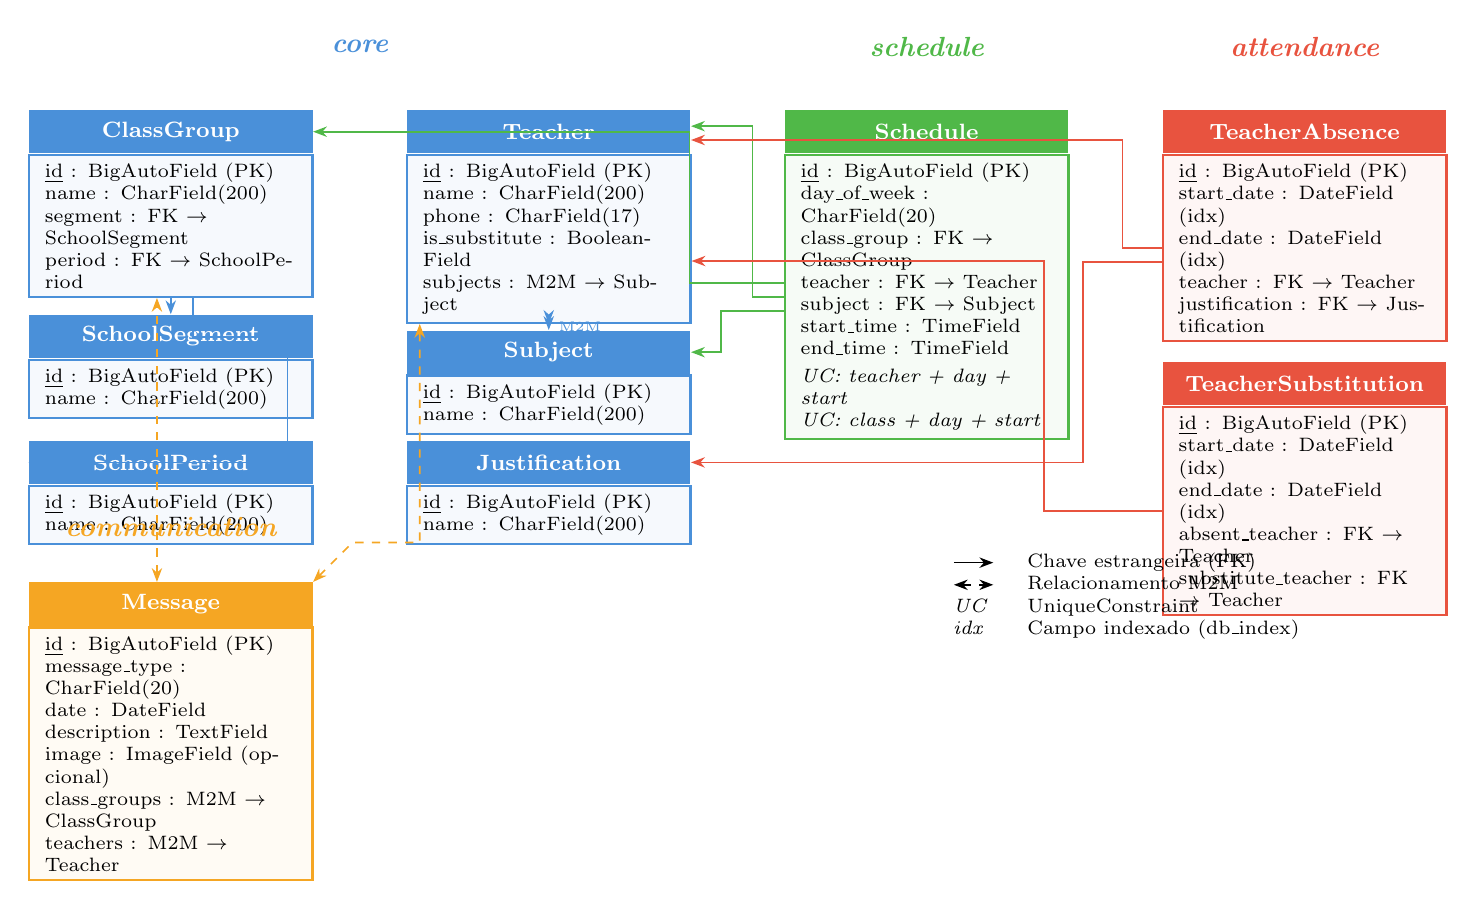
\begin{tikzpicture}[node distance=0.8cm and 1.2cm]

% ── COLUMN 1: CORE LEFT (ClassGroup, Segment, Period) ──────────────

\entityNode{classgroup}{coreColor}{ClassGroup}{%
    \underline{id} : BigAutoField (PK)\\
    name : CharField(200)\\
    segment : FK $\rightarrow$ SchoolSegment\\
    period : FK $\rightarrow$ SchoolPeriod
}{0, 0}

\entityNode{segment}{coreColor}{SchoolSegment}{%
    \underline{id} : BigAutoField (PK)\\
    name : CharField(200)
}{0, -2.6}

\entityNode{period}{coreColor}{SchoolPeriod}{%
    \underline{id} : BigAutoField (PK)\\
    name : CharField(200)
}{0, -4.2}

% ── COLUMN 2: CORE CENTER (Teacher, Subject, Justification) ───────

\entityNode{teacher}{coreColor}{Teacher}{%
    \underline{id} : BigAutoField (PK)\\
    name : CharField(200)\\
    phone : CharField(17)\\
    is\_substitute : BooleanField\\
    subjects : M2M $\rightarrow$ Subject
}{4.8, 0}

\entityNode{subject}{coreColor}{Subject}{%
    \underline{id} : BigAutoField (PK)\\
    name : CharField(200)
}{4.8, -2.8}

\entityNode{justification}{coreColor}{Justification}{%
    \underline{id} : BigAutoField (PK)\\
    name : CharField(200)
}{4.8, -4.2}

% ── COLUMN 3: SCHEDULE ─────────────────────────────────────────────

\entityNode{schedule}{schedColor}{Schedule}{%
    \underline{id} : BigAutoField (PK)\\
    day\_of\_week : CharField(20)\\
    class\_group : FK $\rightarrow$ ClassGroup\\
    teacher : FK $\rightarrow$ Teacher\\
    subject : FK $\rightarrow$ Subject\\
    start\_time : TimeField\\
    end\_time : TimeField\\[2pt]
    \textit{UC: teacher + day + start}\\
    \textit{UC: class + day + start}
}{9.6, 0}

% ── COLUMN 4: ATTENDANCE ───────────────────────────────────────────

\entityNode{absence}{attColor}{TeacherAbsence}{%
    \underline{id} : BigAutoField (PK)\\
    start\_date : DateField (idx)\\
    end\_date : DateField (idx)\\
    teacher : FK $\rightarrow$ Teacher\\
    justification : FK $\rightarrow$ Justification
}{14.4, 0}

\entityNode{substitution}{attColor}{TeacherSubstitution}{%
    \underline{id} : BigAutoField (PK)\\
    start\_date : DateField (idx)\\
    end\_date : DateField (idx)\\
    absent\_teacher : FK $\rightarrow$ Teacher\\
    substitute\_teacher : FK $\rightarrow$ Teacher
}{14.4, -3.2}

% ── COLUMN 1 BOTTOM: COMMUNICATION ────────────────────────────────

\entityNode{message}{commColor}{Message}{%
    \underline{id} : BigAutoField (PK)\\
    message\_type : CharField(20)\\
    date : DateField\\
    description : TextField\\
    image : ImageField (opcional)\\
    class\_groups : M2M $\rightarrow$ ClassGroup\\
    teachers : M2M $\rightarrow$ Teacher
}{0, -6}

% ── RELATIONSHIPS ──────────────────────────────────────────────────

% Core: ClassGroup -> Segment, Period
\draw[rel=coreColor] (classgroup-body.south) -- ++(0,-0.15) -| (segment-header.north);
\draw[rel=coreColor] ([xshift=8pt]classgroup-body.south) -- ++(0,-0.5) -- ++(1.2,0) |- (period-header.west);

% Core: Teacher M2M Subject
\draw[m2m=coreColor] (teacher-body.south) -- node[right, font=\tiny]{M2M} (subject-header.north);

% Schedule FKs
\draw[rel=schedColor] (schedule-body.west) -- ++(-0.4, 0) |- ([yshift=2pt]teacher-header.east);
\draw[rel=schedColor] ([yshift=-5pt]schedule-body.west) -- ++(-0.8, 0) |- (subject-header.east);
\draw[rel=schedColor] ([yshift=5pt]schedule-body.west) -- ++(-1.2, 0) |- (classgroup-header.east);

% Attendance FKs
\draw[rel=attColor] (absence-body.west) -- ++(-0.5, 0) |- ([yshift=-3pt]teacher-header.east);
\draw[rel=attColor] ([yshift=-5pt]absence-body.west) -- ++(-1.0, 0) |- (justification-header.east);
\draw[rel=attColor] (substitution-body.west) -- ++(-1.5, 0) |- ([yshift=-8pt]teacher-body.east);

% Communication M2M
\draw[m2m=commColor] (message-header.north east) -- ++(0.5, 0.5) -| ([xshift=5pt]teacher-body.south west);
\draw[m2m=commColor] ([xshift=-5pt]message-header.north) -- ++(0, 0.3) -| ([xshift=-5pt]classgroup-body.south);

% ── MODULE LABELS ──────────────────────────────────────────────────

\node[module label=coreColor] at (2.4, 0.8) {\normalsize core};
\node[module label=schedColor] at (9.6, 0.8) {\normalsize schedule};
\node[module label=attColor] at (14.4, 0.8) {\normalsize attendance};
\node[module label=commColor] at (0, -5.3) {\normalsize communication};

% ── LEGEND ─────────────────────────────────────────────────────────

\node[anchor=north west, font=\scriptsize] at (9.6, -5.5) {
    \begin{tabular}{ll}
    \tikz\draw[rel=black] (0,0) -- (0.5,0); & Chave estrangeira (FK) \\
    \tikz\draw[m2m=black] (0,0) -- (0.5,0); & Relacionamento M2M \\
    \textit{UC} & UniqueConstraint \\
    \textit{idx} & Campo indexado (db\_index) \\
    \end{tabular}
};

\end{tikzpicture}
\end{document}
